%Centralizar verticalmente.
\newenvironment{midpage}{\vspace*{\fill}}{\vspace*{\fill}}
%Centralizar horizontalmente.
\newenvironment{midline}{\hspace*{\fill}}{\hspace*{\fill}}
\documentclass[12pts]{article}
\usepackage[utf8]{inputenc}
%Pacote para colocar cor no código.
\usepackage{color}
\definecolor{light-gray}{gray}{0.95}
%Pacote para inserir código.
\usepackage{listings}
\lstset{
    numbers=left,
    tabsize=2,
    backgroundcolor=\color{light-gray},
}\title{
	Prática de Eletrônica Digital 1 - (119466)
	\singlespacing
		Turma E (Unb - Gama)
	\singlespacing
	\begin{midpage}
	\begin {large}
		Relatório Experimento 6
		\singlespace
		Introdução ao projeto em FPGA
	\end {large}
	\end{midpage}
}
\date{Outubro 09, 2016}
\usepackage{indentfirst}
\usepackage{setspace}
\usepackage{verbatim}
\usepackage[pdftex]{hyperref}
\usepackage{graphicx}
\begin{document}
\maketitle	
%\vspace{100 mm}
\begin{center}

\begin{tabular}{|c|l|r|}
\hline
Nome & Matrícula & Assinatura\\
\hline

Arthur Temporim & 14/0016759 & \\
\hline	
Eduardo Nunes & 14/0056189 & \\

\hline	
\end{tabular}

\end{center}


\newpage

\section{Sumário}

\begin{itemize}
	\item Introdução
	\singlespacing
	\item Experimentos
	\singlespacing
	\item Discussão
	\singlespacing
	\item Conclusões 
	\singlespacing
	\item Referências Bibliograficas
	\singlespacing
	%\item Diagramas esquemáticos
\end{itemize}

\newpage


\section{Introdução}
\iffalse
Introdução, indicando a delimitação do tema, apresentando a justificativa descrevendo o propósito do relatório.
\fi

\section{Experimentos}
\iffalse
Parte Experimental, descrevendo os passos realizados, dificuldades e soluções para os problemas encontrados. Aqui, deve-se apresentar uma descrição dos resultados encontrados em forma de figuras, gráficos e tabelas.
\fi

	Neste relatório é apresentado o resultado obtido com o projeto na FPGA realizados na aula prática de eletrônica digital 1. Estes resultados são expostos através de imagens e comentários a respeito do experimento. 

\subsection{Experimento 01}
\singlespacing
	O primeiro experimento, tratou-se de projetar o código em VHDL, feito no pré-relatório 6, na FPGA utilizando o software \textit{Vivado}. 

	Os primeiros passos seguidos tratou se de configurar o ambiente para identificar no software qual modelo de FPGA utilizaríamos sendo este o: Basys 3. Portanto, senguindo os passos que foram passados em sala, conseguimos criar um novo projeto e fazer as devidas configurações necessárias para que o software reconhece se o modelo da FPGA. Porém, antes de concluir estes procedimentos, de forma inesperada, fomos muito prejudicados pelo computador e pelo alto acesso ao servidor que deixou o processo extremamente lento, levando se mais ou menos 40 minutos para que a máquina aplica se as configurações desejadas, isto contando o tempo em que ela começou a processar e o tempo em que ela travou 3 vezes durante este processo. 
	
	Mesmo com este imprevisto conseguimos passar para a segunda parte do experimento, que seria projetar o código VHDL na FPGA Basys 3. Então, utilizando o código que havíamos projetado no pré-relatório 6, iniciamos os devidos procedimentos. Porém, ocorreu outro erro inesperado, no momento em que sintetizaríamos o código aparecia as seguintes mensagens de erro:

\clearpage
\begin{figure}[!htb]
  \centering
  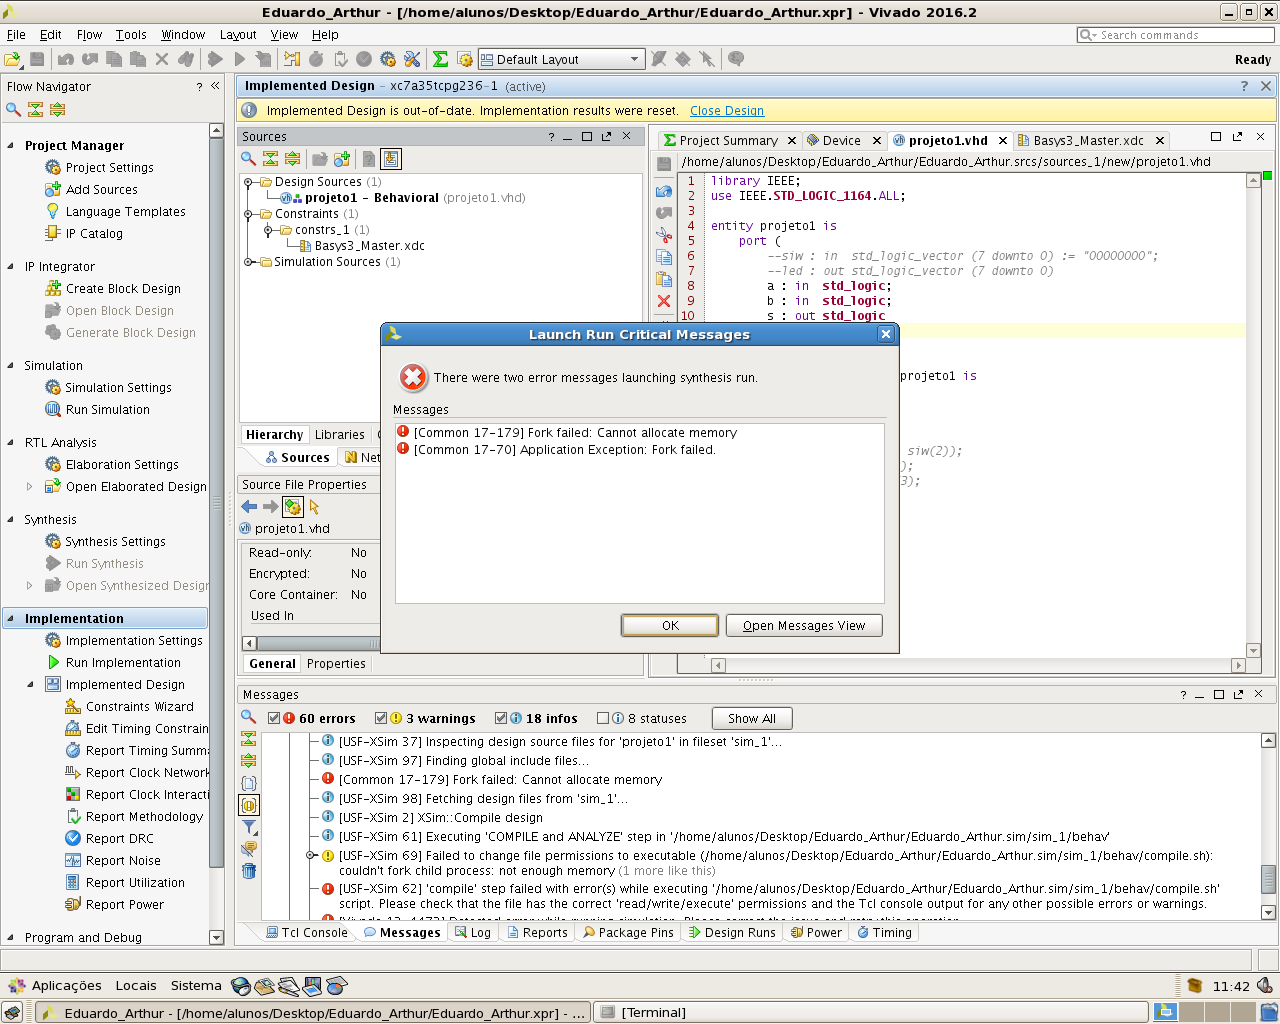
\includegraphics[scale=0.30]{imagens/tretaMemoria.png}
  \caption{Mensagens do primeiro erro - Vivado}	
  \label{figRotulo}
\end{figure}

\clearpage
\begin{figure}[!htb]
  \centering
  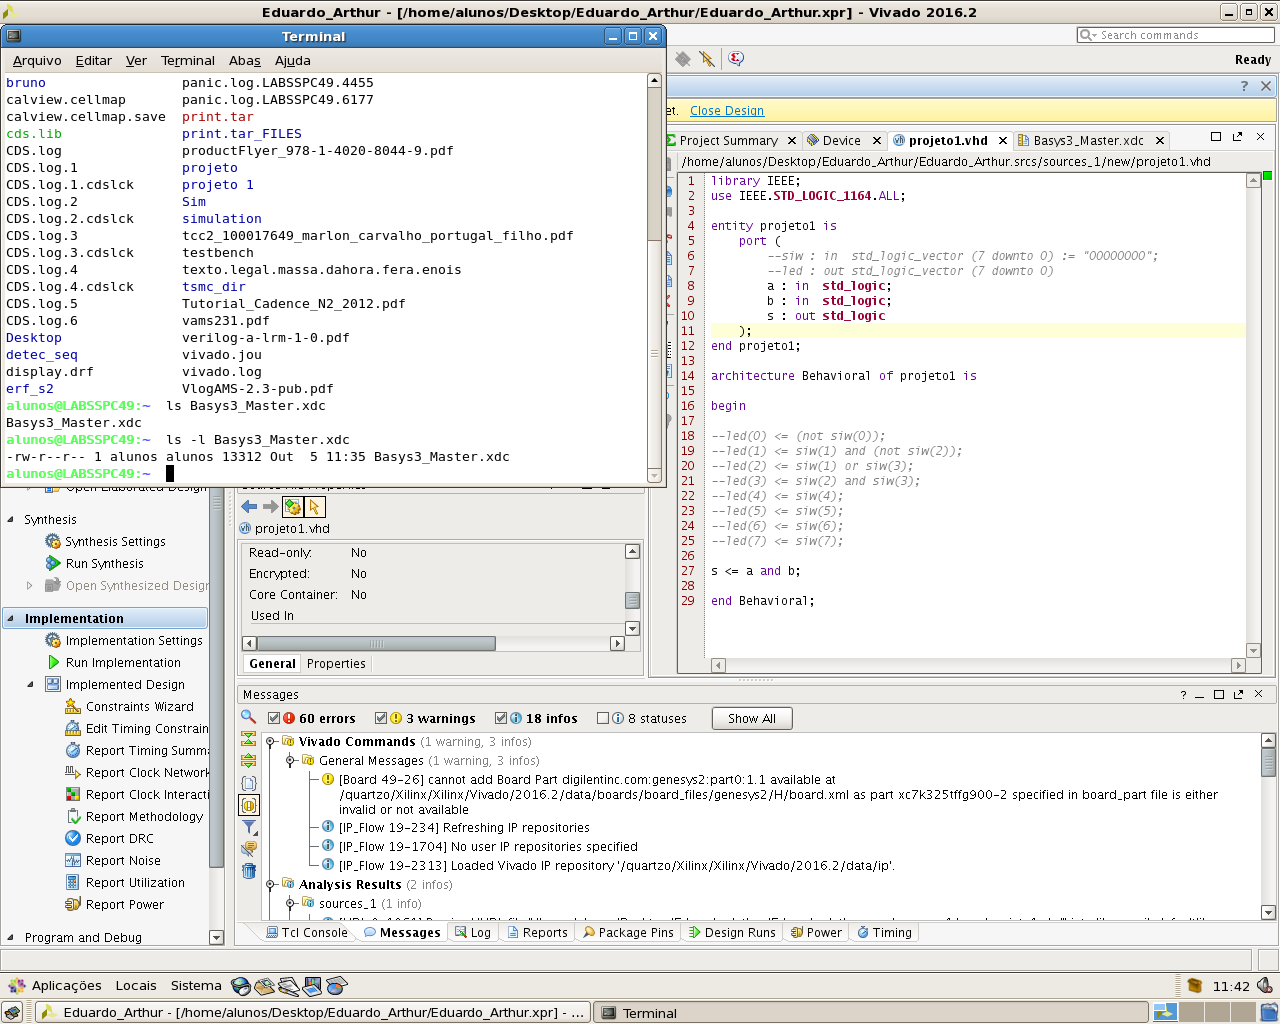
\includegraphics[scale=0.30]{imagens/tretaPermissao.png}
  \caption{Mensagens do segundo erro - Vivado}	
  \label{figRotulo}
\end{figure}
	
	Pensando assim em solucionar o problema, achamos que este poderia ser o código, apesar do código no pré relatório 6 ter funcionado sem nenhum tipo de problema. Então, tentamos fazer um código simples implementando somente uma porta AND. Mas, uma tentiva sem exito, a mensagem continuou a ocorrer. Pedimos ajuda ao monitor e aos professores, porém ninguém conhecia a causa deste tipo de erro. Então, foi concluído que o problema estava na máquina.  


\section{Discussão}
\iffalse
Discussão sobre os resultados encontrados, comentando detalhadamente as medições realizadas e dando a devida interpretação destas, informando se os objetivos da experimento foram alcançados. Esta é uma das partes mais importantes do relatório: aqui, há oportunidade para expressar os conhecimentos adquiridos na prática e fazer a interrelação com os fundamentos teóricos.
\fi
      Neste sexto relatório não foi possível realizar o experimento com êxito devido aos fatores apresentados acima. Ficamos muito frustrados com este resultado, porém já tomamos medidas para que estes tipos de imprevistos não ocorram novamente e nos prejudique como prejudicou neste experimento seis.

\section{Conclusões}
\iffalse
Conclusões, mostrando os êxitos e eventuais problemas encontrados na realização do experimento, indicando as limitações, apresentando recomendações e/ou sugestões.
\fi

Com a realização deste experimento não conseguimos obter resultados positivos. Porém, ganhamos experiência para poder tentar evitar estes tipos de imprevistos e acabamos por entender a parte teórica do funcionamento da FPGA, conhecimento este passado na aula prática e na realização do pré relatório 06. 

\section{Referências Bibliográficas}
\iffalse
Referencias Bibliográficas, relacionadas e citadas de acordo com as normas da ABNT.
\fi
Prática de Eletrônica Digital I 2016.2 professores Henrique Marra Taira Menegaz,Leonardo Aguayo, Lourdes Mattos Brasil, Marcus Vinícius Chaffim Costa, Mariana Costa Bernardes Matias. UnB - FGA Agosto de 2015.

\iffalse
\section{Diagramas Esquemáticos}
Diagramas Esquemáticos. Todos os diagramas devem ser inseridos ao final do relatório em páginas separadas do texto, indicando a identificação do circuito, autor, revisor, versão e datas relevantes.
\fi
\newpage

\end{document}

%Exemplo de imagem
\iffalse
\begin{figure}[!htb]
  \centering
  \includegraphics[scale=0.3	]{nome_da_imagem}
  \caption{Descrição}
  \label{figRotulo}
\end{figure}
\fi

% Exemplo de tabela.
\iffalse
\begin{tabular}{|c|r|}
\hline
Material Utilizado & Quantidade\\
\hline
Cabo Banana-Banana & 2  \\
\hline
Fios de cobre & x \\
\hline
Cabo coaxial & 3  \\
\hline
CI 74HC00   & 1 \\
\hline
CI 74LS00   & 1 \\
\hline
Protoboard & 2 \\
\hline
Fonte de tensão MPL-3305M & 1 \\
\hline	
Multímetro Digital  & 1 \\
\hline
Gerador de funçoes iCEL modelo GV-2002 & 1 \\
\hline
Osciloscopio BK 2530 & 1 \\
\hline
\end{tabular}
\singlespacing
\fi

